\documentclass{article}
\usepackage[utf8]{inputenc}
\usepackage[spanish]{babel}
\usepackage{listings}
\usepackage{graphicx}
\graphicspath{ {images/} }
\usepackage{cite}

\begin{document}

\begin{titlepage}
    \begin{center}
        \vspace*{1cm}
            
        \Huge
        \textbf{Implementación y Diseño}
            
        \vspace{0.5cm}
        \LARGE
        StonerIt (Proyecto Final)
            
        \vspace{1.5cm}
            
        \textbf{Nelson Fernando Parra Guardia}
            
        \vfill
            
        \vspace{0.8cm}
            
        \Large
        Departamento de Ingeniería Electrónica y Telecomunicaciones\\
        Universidad de Antioquia\\
        Medellín\\
        Octubre de 2021
            
    \end{center}
\end{titlepage}

\newpage
\section{Diseño}
Para el proyecto final, inicialmente se plantean 5 niveles: dos de los cuales tendrán enemigos normales (pequeños y múltiples) y tres de ellos serán jefes. De igual manera, se postulan los siguientes mapas, donde el bloque A será el borde de la ventana (que todos los mapas tendrán) y el bloque B, uno indestructible que le impedirá movimiento y ataques al jugador. Los mapas de las figuras 2 y 3, pertenecerán a los niveles 1 y 3 en los cuales hay que luchar con enemigos normales (explicados anteriormente) y los niveles que contengan un jefe, se van a desenvolver en un mapa abierto sin obstáculos.

\begin{figure}[h]
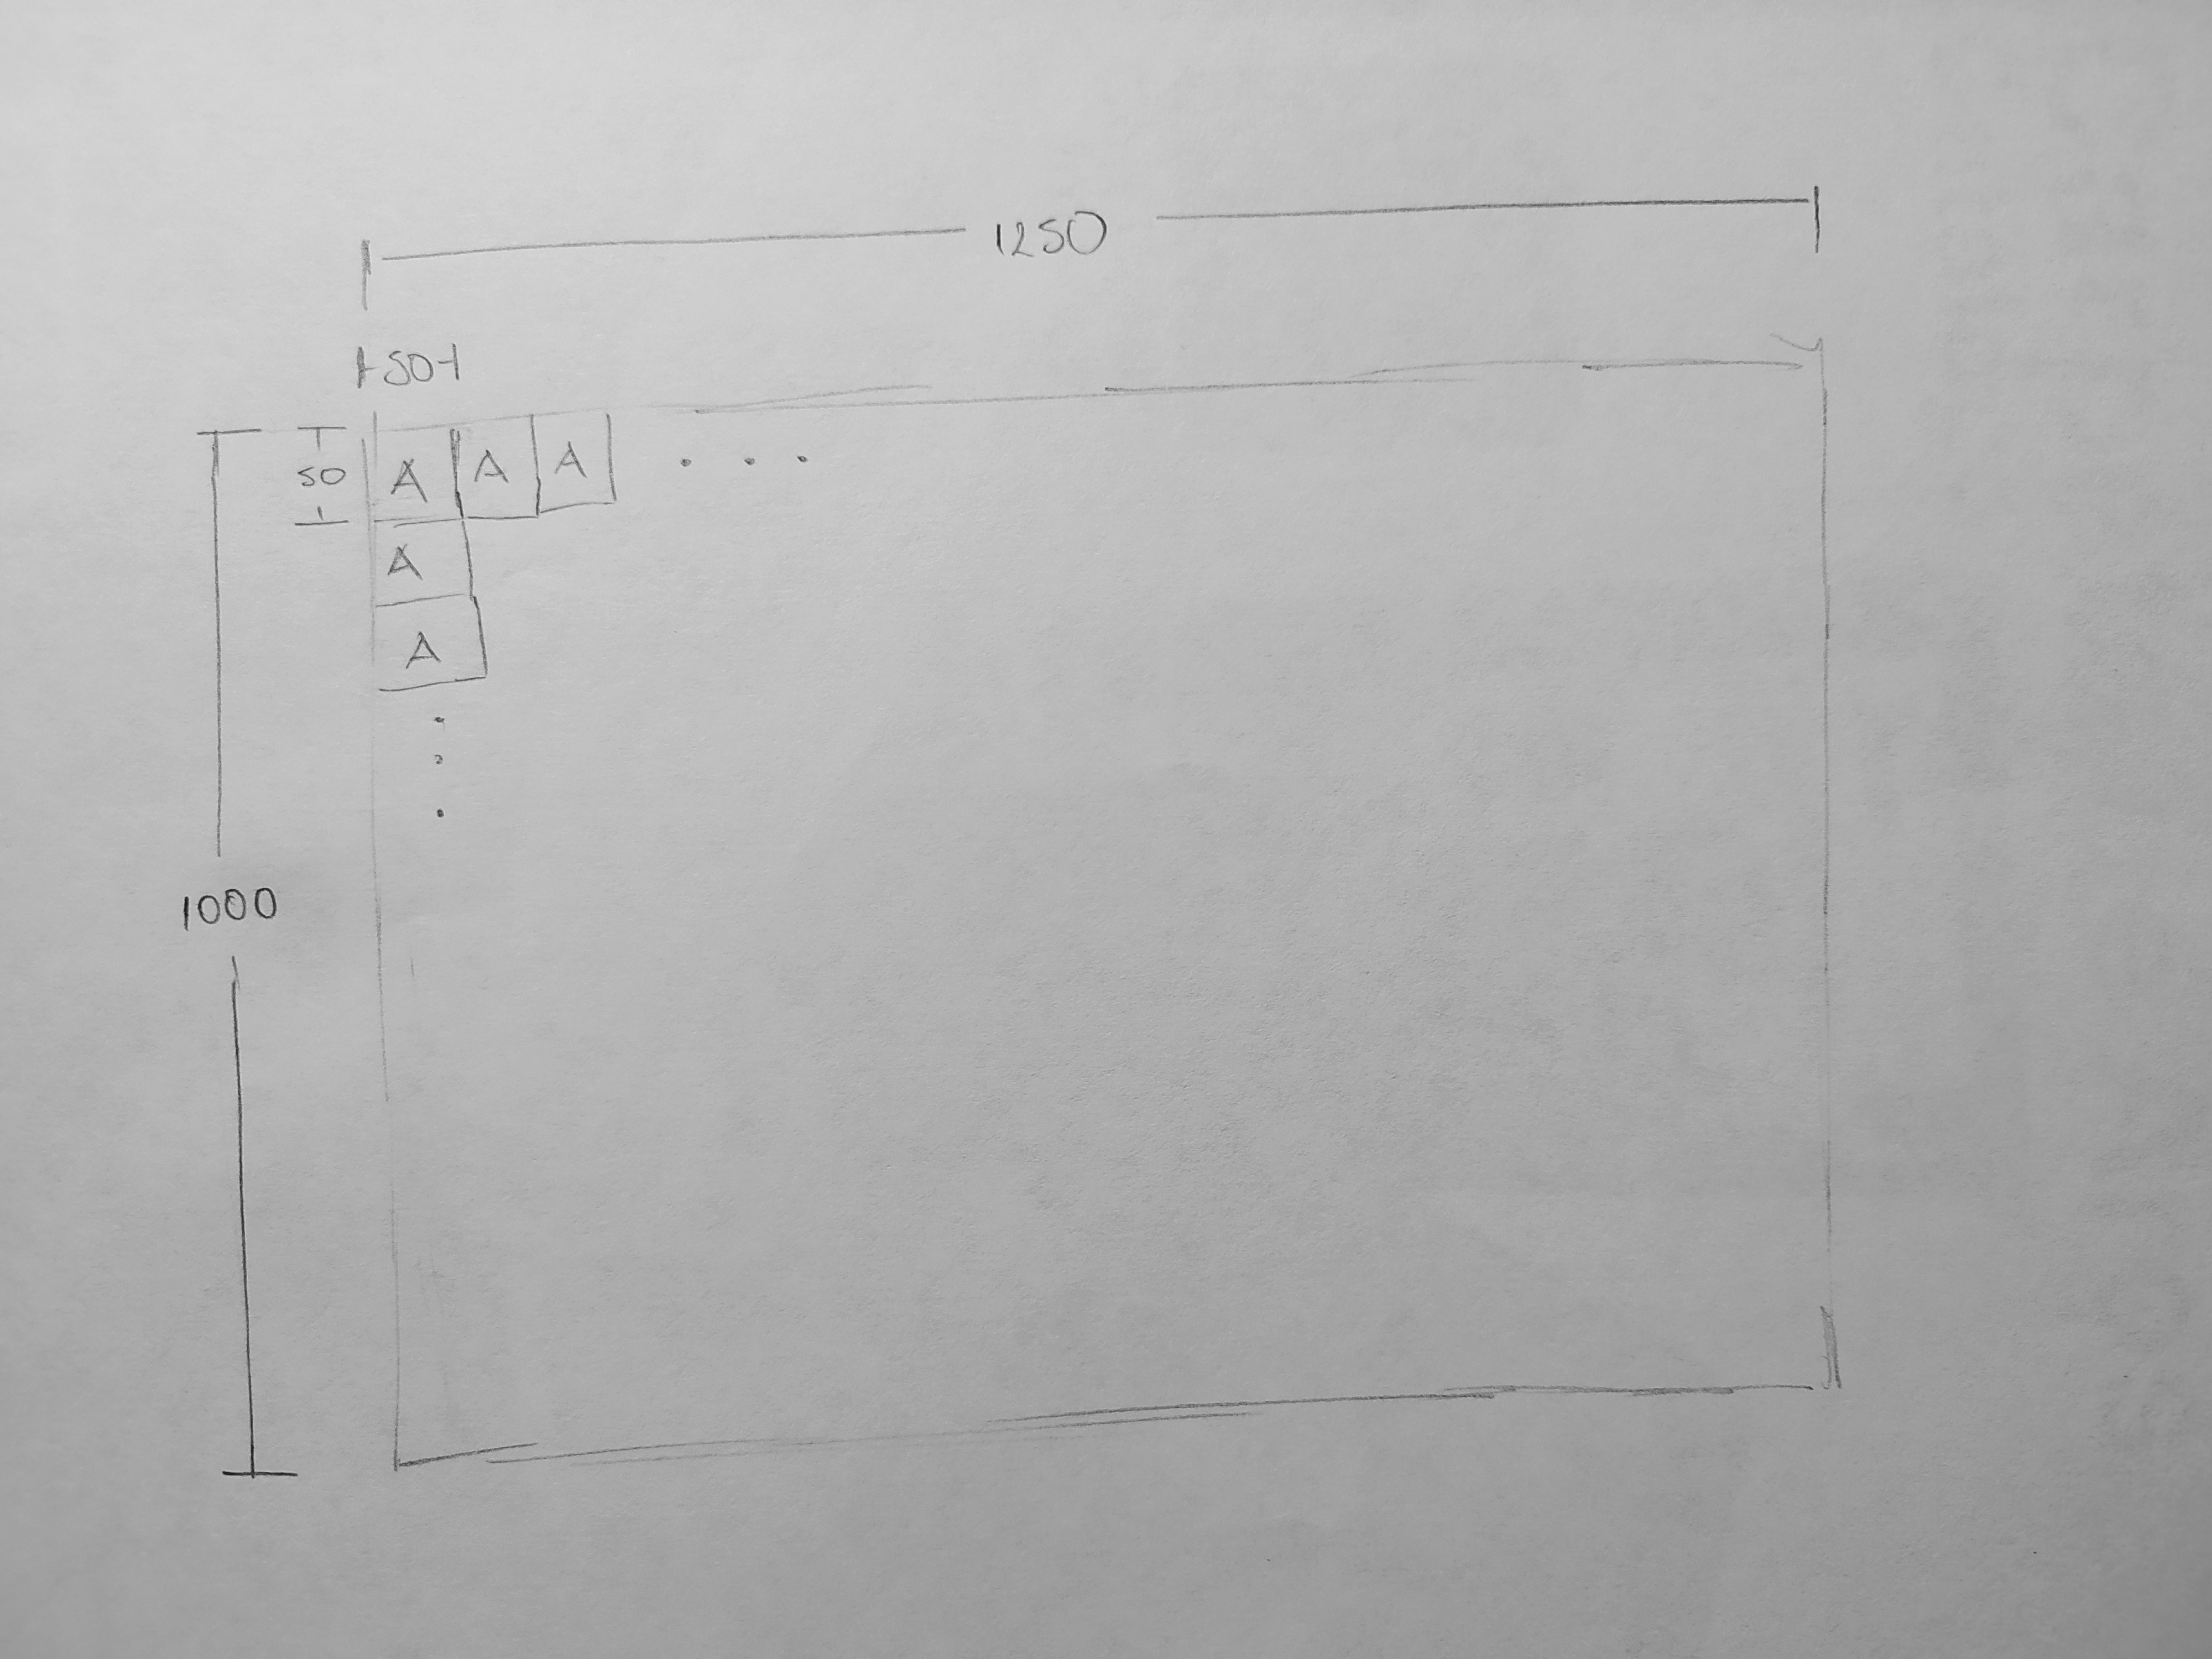
\includegraphics[width=10cm, height=5cm]{imagenes/bordes.jpg}
\centering
\caption{Contorno de los mapas.}
\end{figure}

\begin{figure}[h]
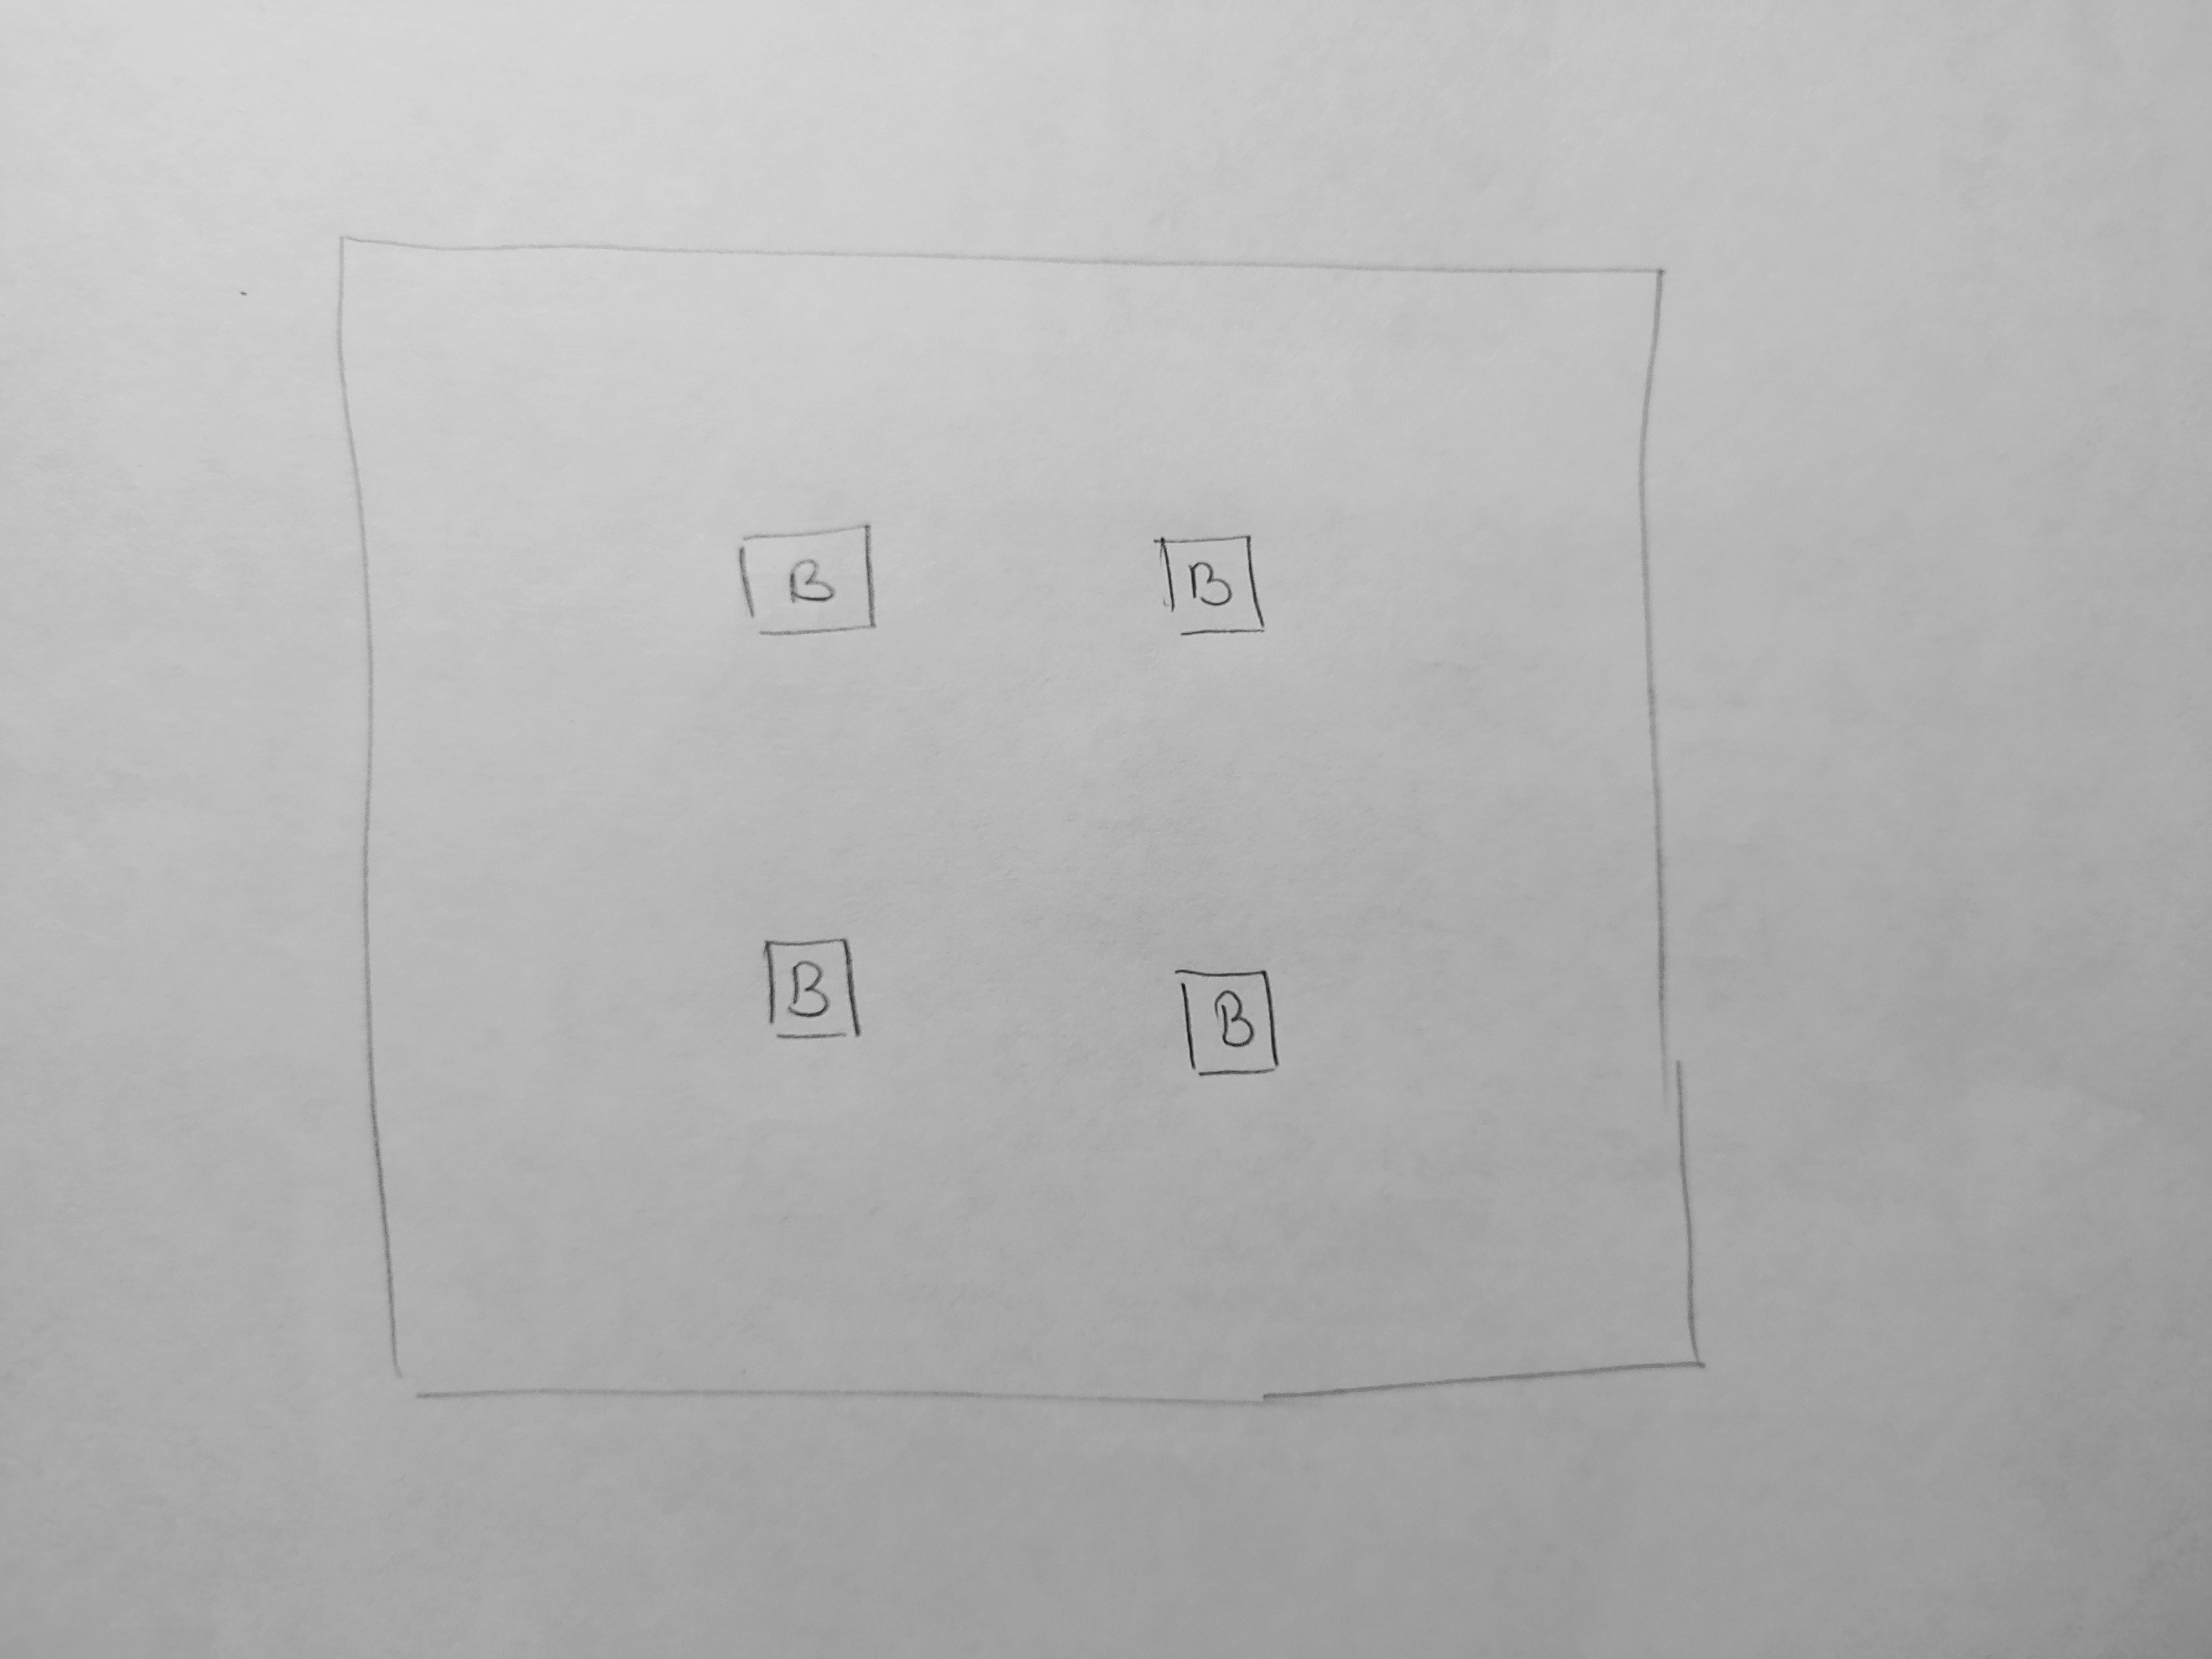
\includegraphics[width=10cm, height=5cm]{imagenes/mapa1.jpg}
\centering
\caption{Mapa nivel 1.}
\end{figure}

\begin{figure}[h]
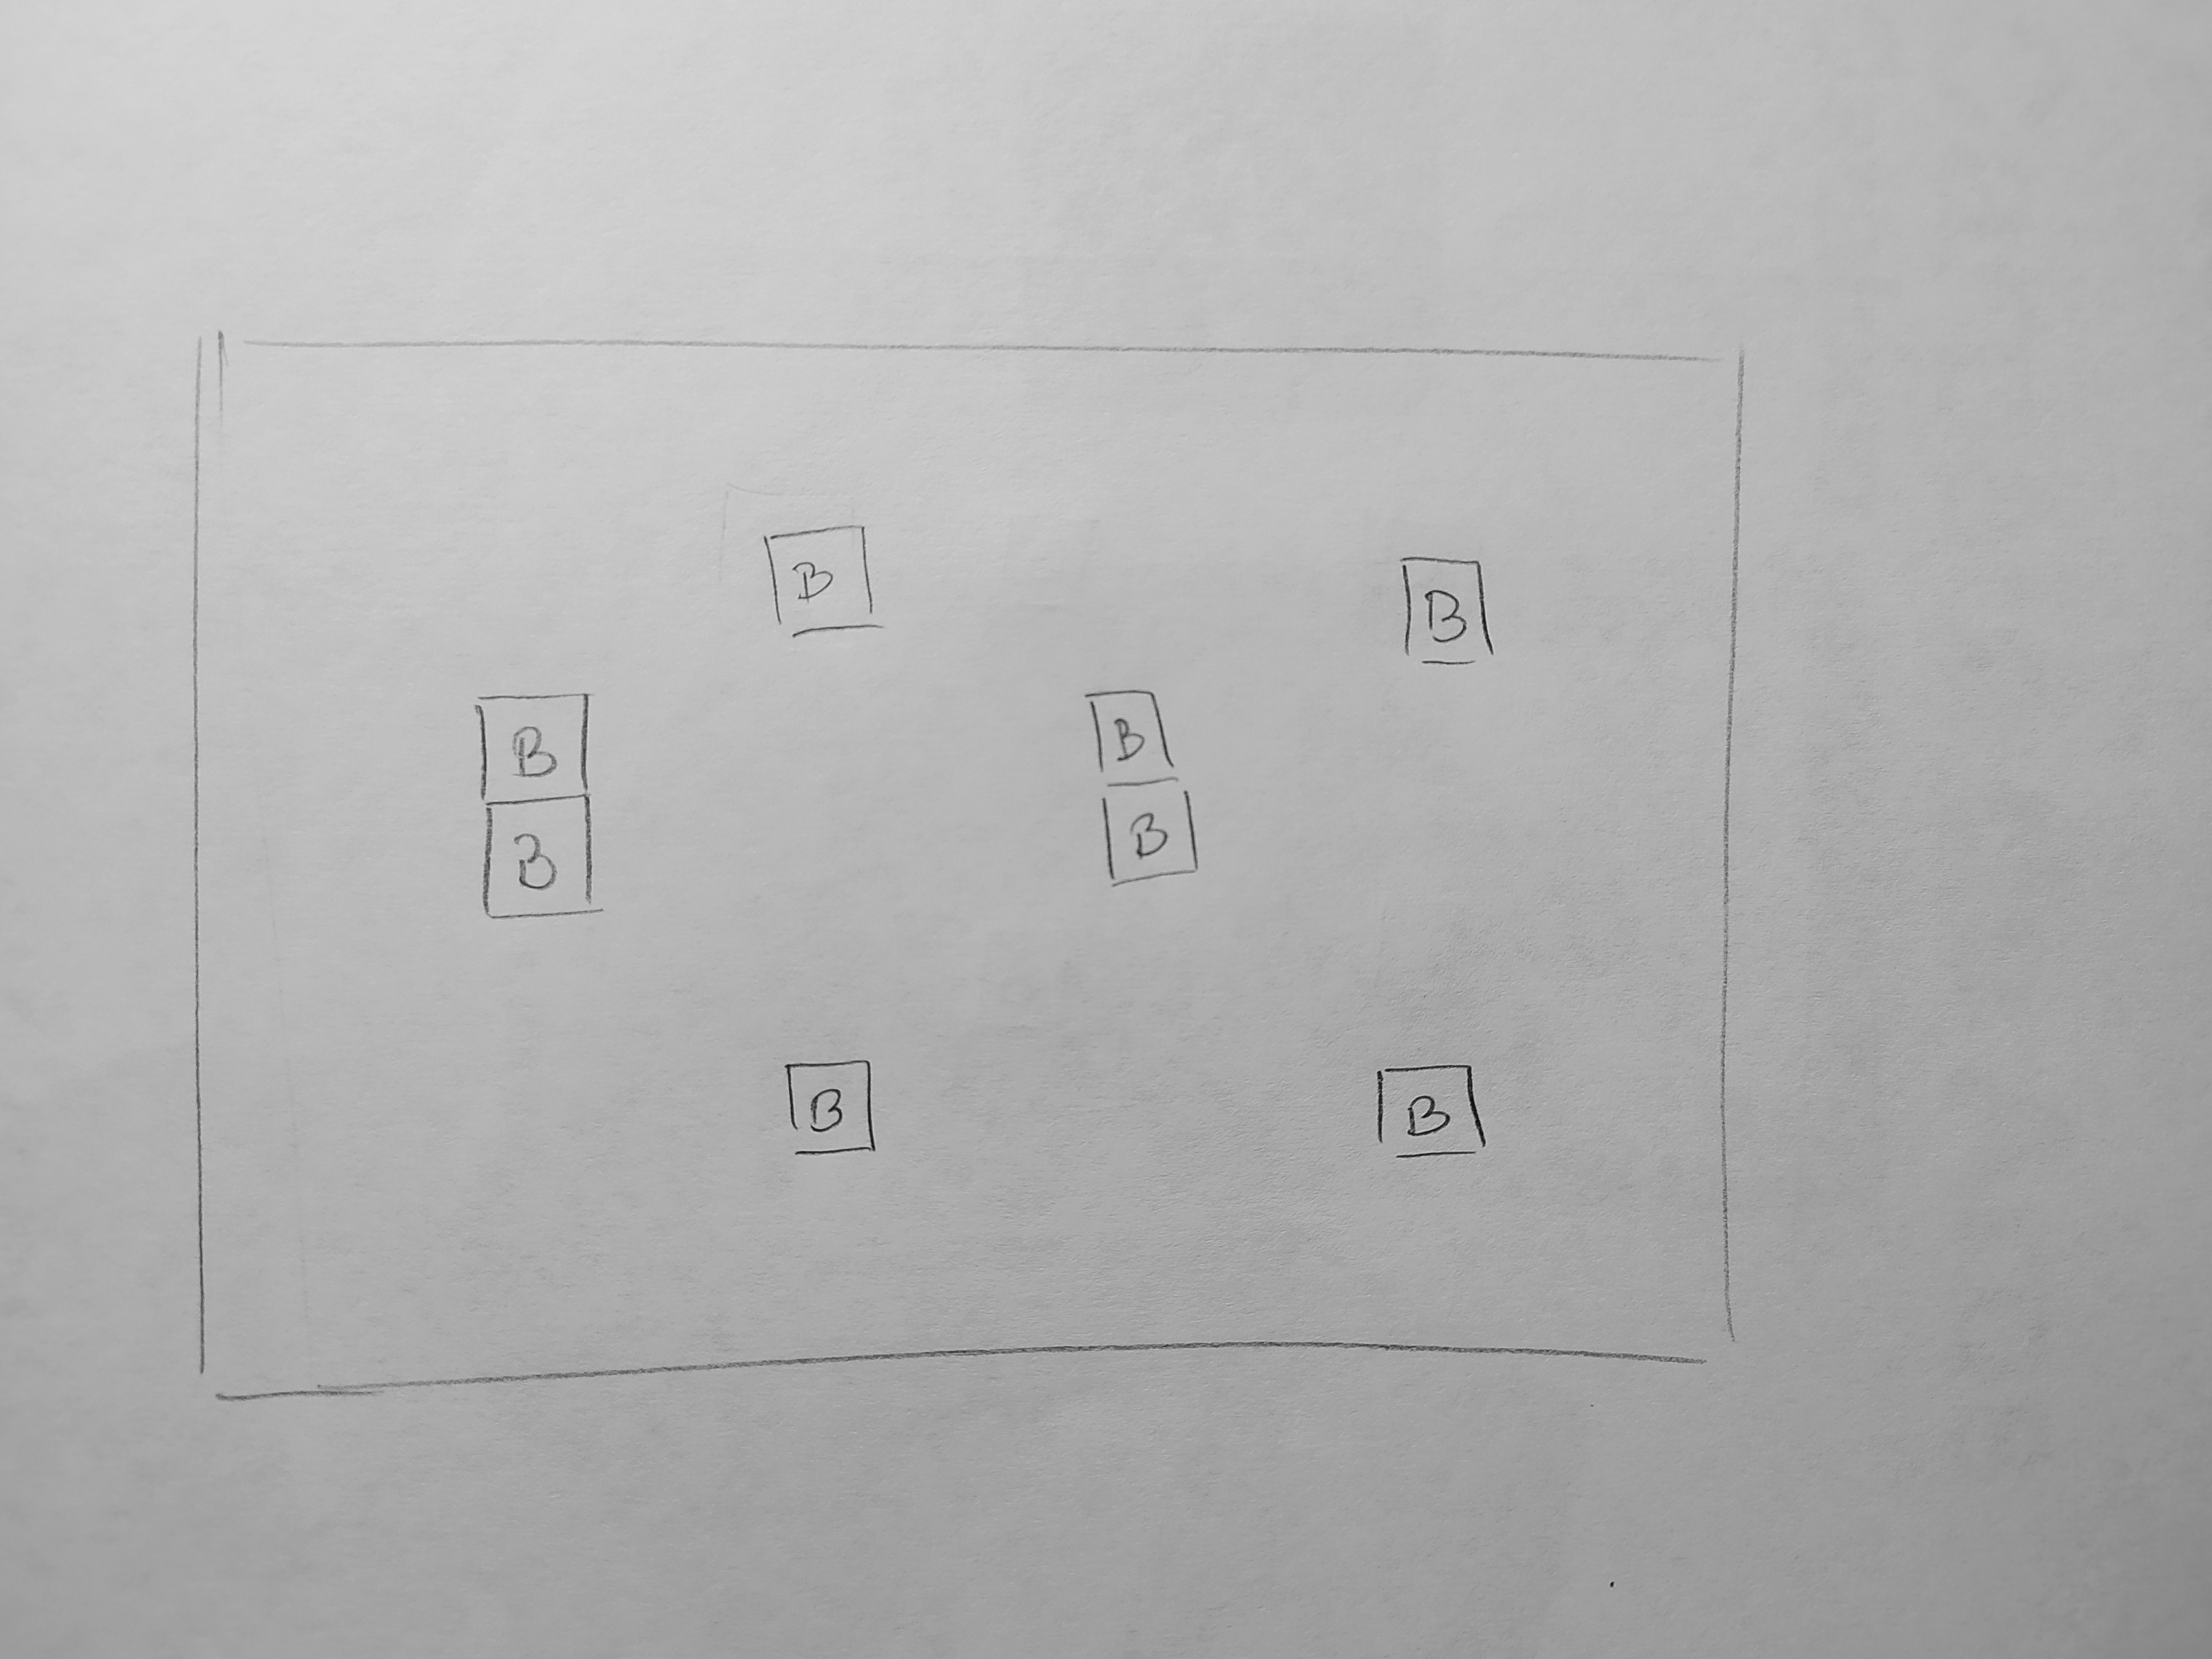
\includegraphics[width=10cm, height=5cm]{imagenes/mapa3.jpg}
\centering
\caption{Mapa nivel 3.}
\end{figure}

\newpage
\subsection{Bloques A}
\par En orden de nivel:
\begin{figure}

\includegraphics[width=12cm]{imagenes/bloquesa.png}
\centering
\end{figure}

\subsection{Bloques B}
\par En orden de nivel:
\begin{figure}[h]

\includegraphics[width=5cm]{imagenes/bloquesb.png}
\centering
\caption{Bloques B.}
\end{figure}

\newpage
\subsection{Personaje y poder}
\par En orden de nivel:
\begin{figure}[h]

\includegraphics[width=2.5cm]{imagenes/PERSONAJE.png}
\centering
\caption{Personaje.}
\end{figure}

\subsection{Enemigos y poderes}
\par En orden de nivel:
\begin{figure}[h]

\includegraphics[width=12cm]{imagenes/villanos.png}
\centering
\caption{Enemigos.}
\end{figure}

\section{Inconvenientes}
De primeras, uno de los impedimentos que se me presenta es el hecho de colocar niveles y múltiples escenas a una misma ventana. Sin embargo, sin pensarlo mucho, se plantea que cada vez que una escena termine su función (menú o juego) todos los ítems de la escena se eliminan y se crean unos nuevos con la utilidad siguiente.
\par Luego de haber meditado bastante la idea, revisando el código y con el conocer que se pueden crear distintas escenas en el programa, se propone crear varias de éstas para cada pantalla que se requiera (inicio, niveles, etc.) y, luego, mostratrlas con \textsl{ui-$>$graphicsView-$>$setScene($<$escena$>$);}.

\section{Cronograma}
\begin{figure}[h]
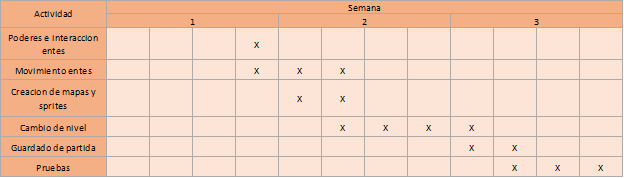
\includegraphics[width=12cm]{imagenes/cronograma.png}
\centering
\caption{Cronograma de la implementación.}
\label{fig:diagram}
\end{figure}

\end{document}
